% !TeX spellcheck = en_US
%\documentclass[11pt,a4paper]{article}
\documentclass[11pt
  , a4paper
  , article
  , oneside
%  , twoside
%  , draft
]{memoir}

\usepackage{control}
\usepackage[numbers]{natbib}


\begin{document}

\newcommand{\technumber}{
  RAON Control-Document Series\\
  Revision : v1.0,   Release : 2015-03-16 fixed date}
\title{\textbf{Matlab-Simulink, Vivado-System Generator 개발환경 구축}}

\author{이상일\thanks{silee7103@ibs.re.kr}, 손창욱 \\

  Rare Isotope Science Project\\
  Institute for Basic Science, Daejeon, South Korea
}
\date{\today}
\renewcommand{\maketitlehooka}{\begin{flushright}\textsf{\technumber}\end{flushright}}
%\renewcommand{\maketitlehookb}{\centering\textsf{\subtitle}}
%\renewcommand{\maketitlehookc}{C}
%\renewcommand{\maketitlehookd}{D}

\maketitle

\begin{abstract}
FPGA가 적용된 시스템은 MRF Timing System, Fast Protection System, 고속 Stepper Motor Control System Prototype을 비롯한 시스템이 있으며, 향 후 에는 FPGA가 적용되는 Control System이 증가 할 것으로 예상된다. FPGA 개발은 HDL(Hardware Description Language) 언어를 사용하여 설계하게 되는데 그에 대한 내용이 방대하며, 개발 또한 쉽지 않다. 
이런 환경에서 좀더 개발기간과 FPGA 설계를 위한 부분을 가속하기 위하여 Matlab-Simulink의 HDL Coder를 활용 한다. 본 문서는 Matlab-Simulink HDL Coder를 사용하여 FPGA를 개발하기 위한 절차를 문서화 하기 위함이다.
\end{abstract}

\clearpage

\chapter{FPGA - Simulink 설치}
FPGA(Field Programmable Gate Array)는 Hardware의 IC 소자의 gate array를 사용자가 program하여 회로를 구성할 수 있는 chip을 말한다. FPGA 프로그램 개발은 HDL(Hardware Description Language) 개발표준 언어를 사용하며 프로그램 할 수 있으며 아래와 같은 두 가지 HDL 언어를 지원한다.

\begin{itemize}
	\item VHDL
	\item Verilog HDL
\end{itemize}

HDL를 이용한 개발의 효율성을 증대하기 위하여 Matlab-Simulink를 설치 및 사용한다. Matlab은 RAON에서 Standalone 형태의 개발 라이센스를 포함한다. Matlab 버젼은 matlab\_R2014a\_glnxa64 버전을 다운받아 아래와 같은 절차로 설치한다.

\begin{figure}[h!]
	\centering
	\includegraphics[width=0.8\textwidth, height=0.4\textwidth]{./images/matlab-1.eps}
	\caption{Procedure Matlab installation}
	\label{fig:install_1} 
\end{figure}
\begin{figure}[h!]
	\centering
	\includegraphics[width=0.8\textwidth, height=0.4\textwidth]{./images/matlab-2.eps}
	\caption{Procedure Matlab installation}
	\label{fig:install_2} 
\end{figure}
Email address:silee7103@ibs.re.kr, Password:dE~D
\hfil\break

\begin{figure}[h!]
	\centering
	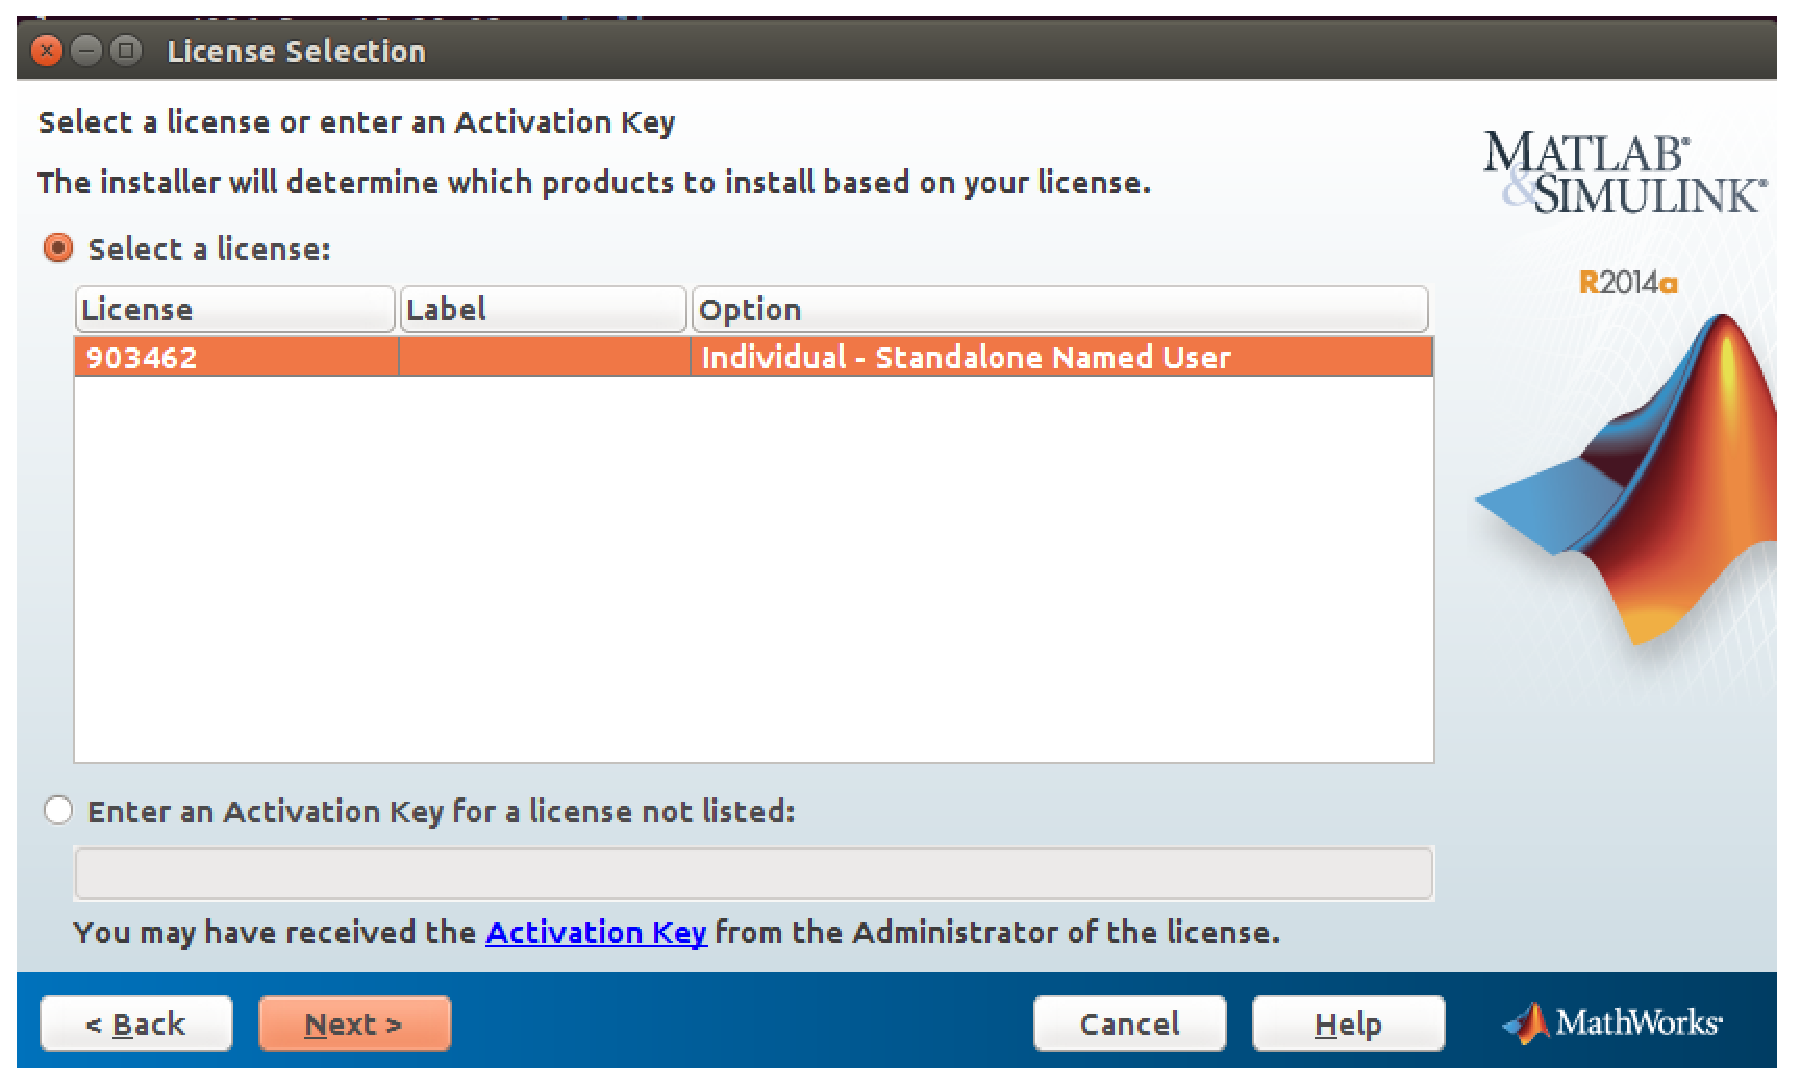
\includegraphics[width=0.8\textwidth, height=0.4\textwidth]{./images/matlab-3.eps}
	\caption{Procedure Matlab installation}
	\label{fig:install_3} 
\end{figure}	


\begin{figure}[h!]
	\centering
	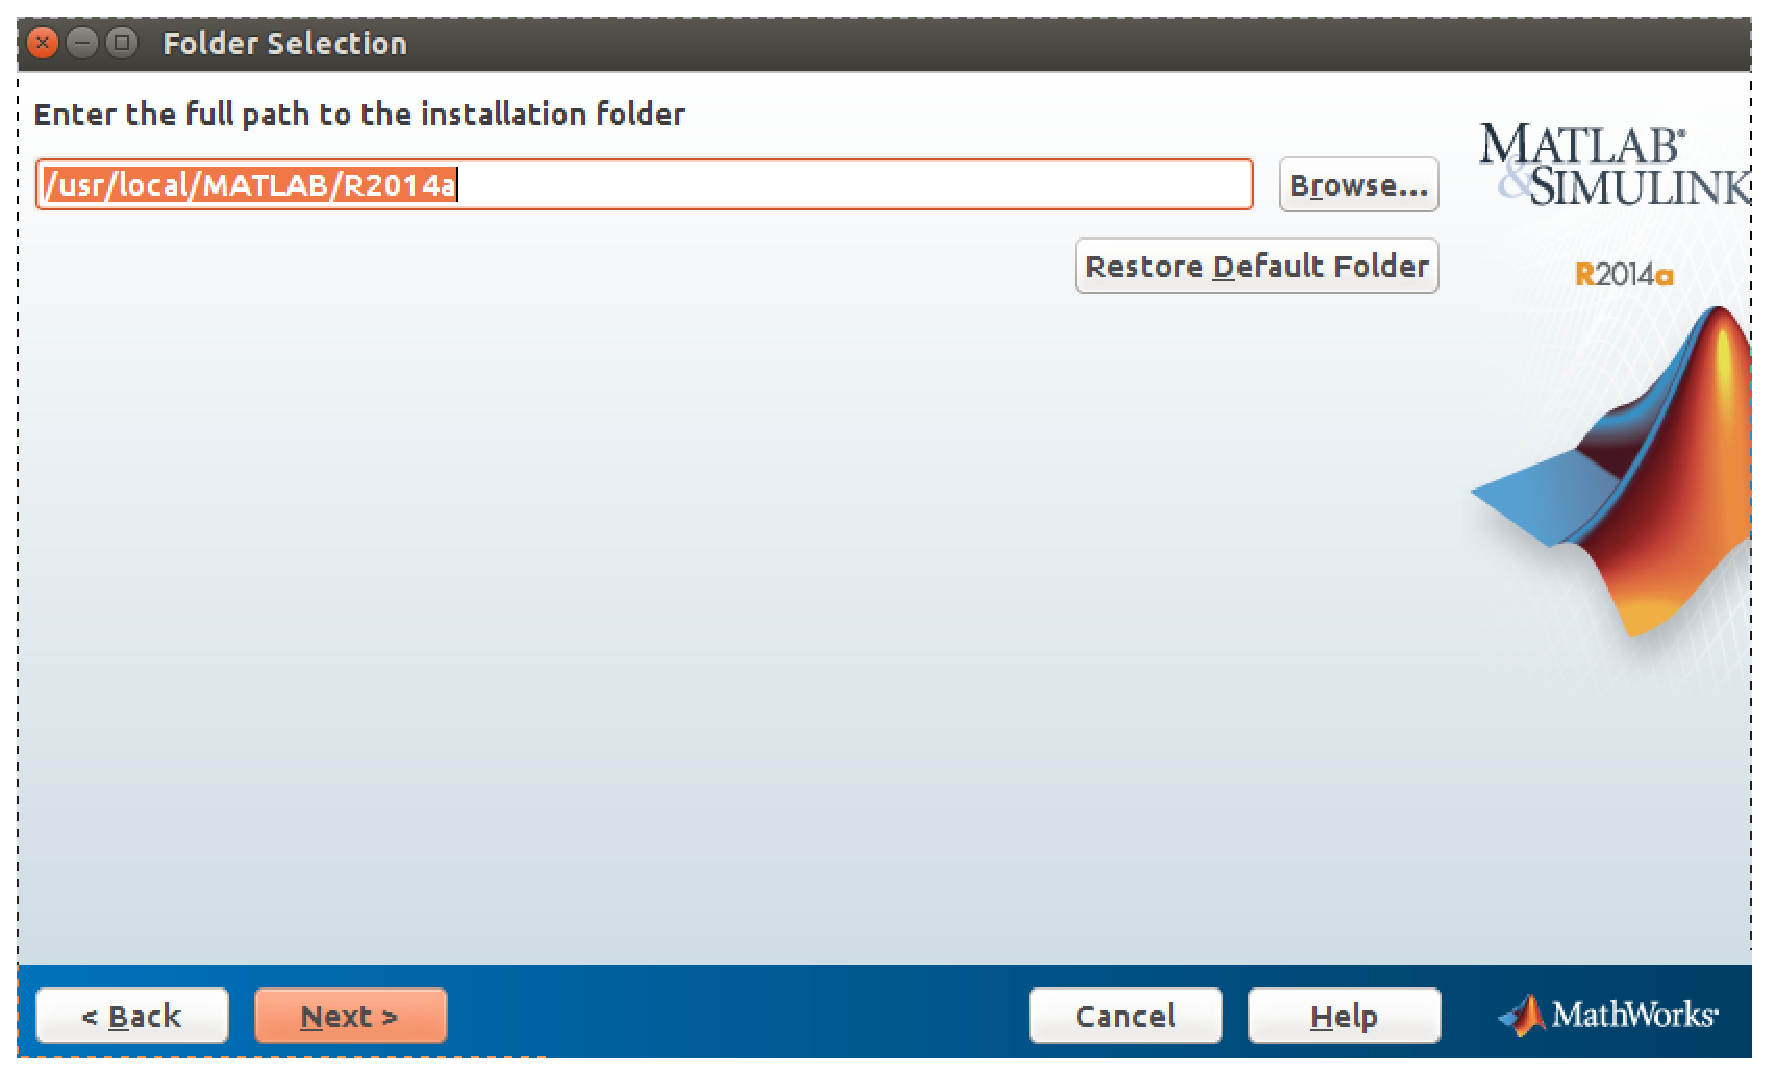
\includegraphics[width=0.8\textwidth, height=0.4\textwidth]{./images/matlab-4.eps}
	\caption{Procedure Matlab installation}
	\label{fig:install_4} 
\end{figure}	


\begin{figure}[h!]
	\centering
	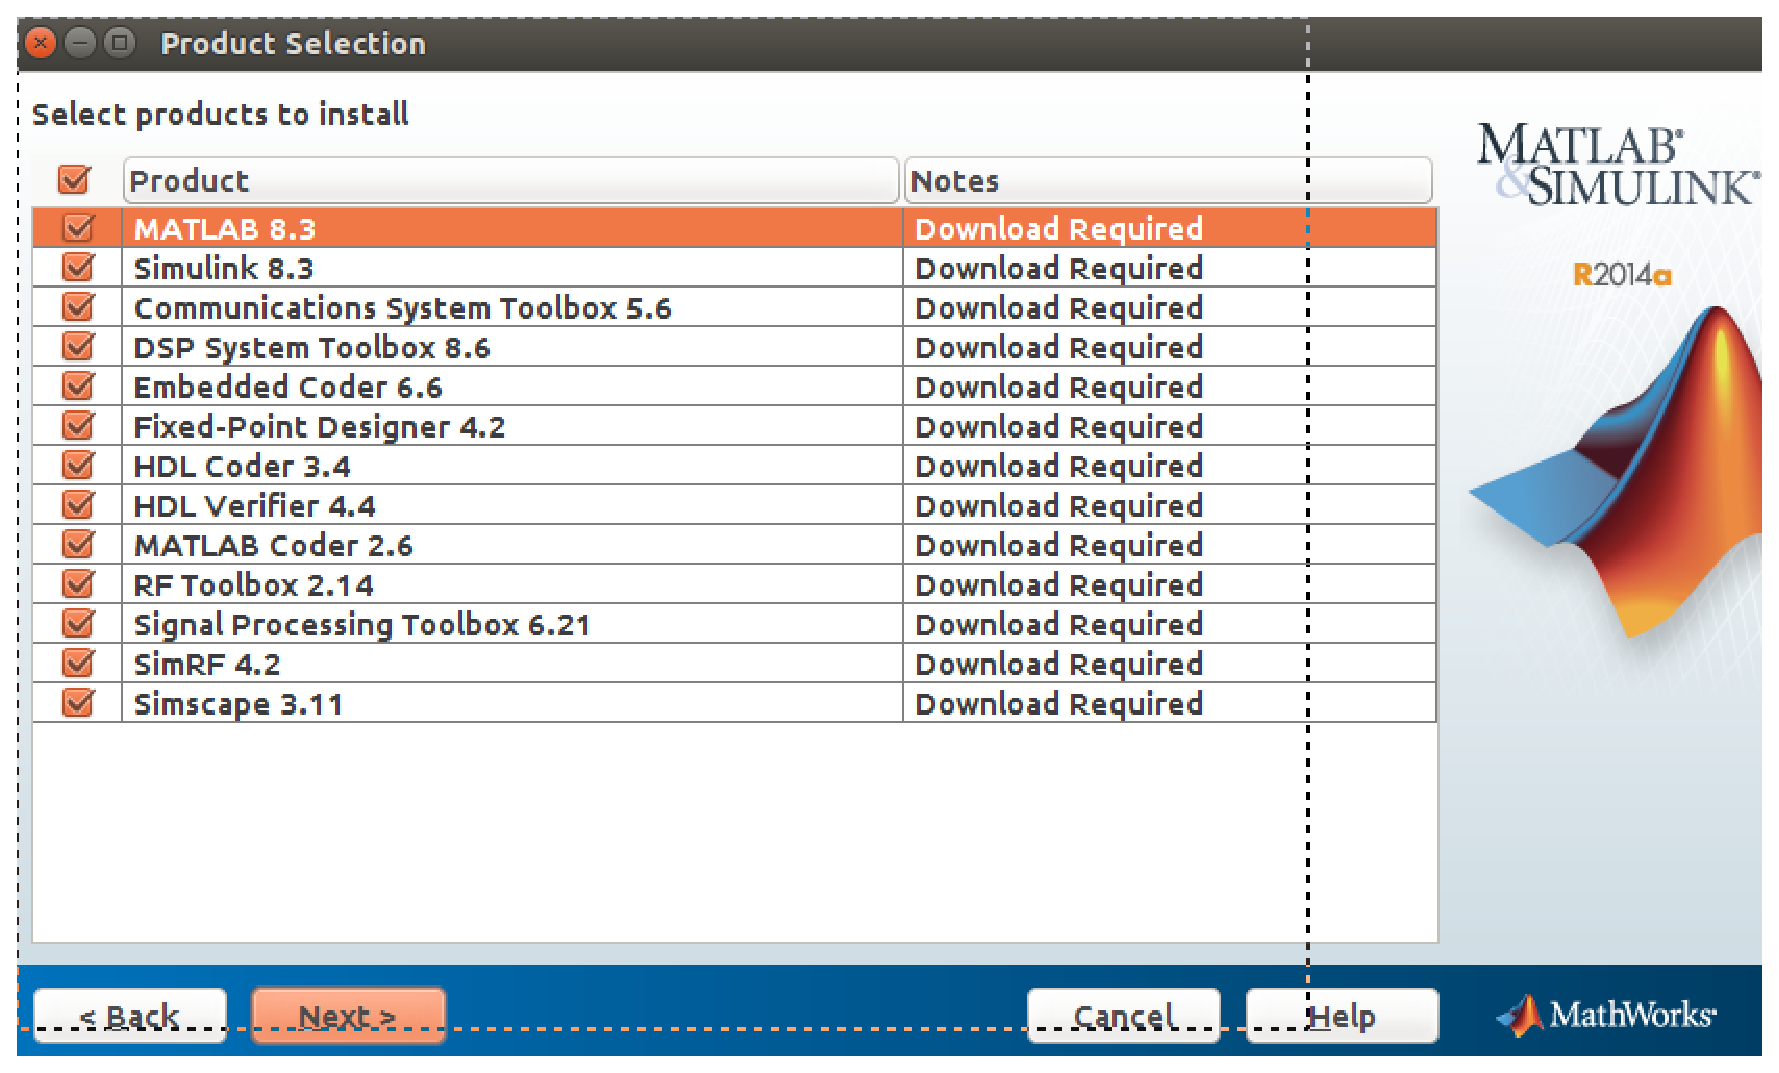
\includegraphics[width=0.8\textwidth, height=0.4\textwidth]{./images/matlab-5.eps}
	\caption{Procedure Matlab installation}
	\label{fig:install_5} 
\end{figure}	

Matlab에서 사용할 수 있는 라이센스를 확인한다.  여기에 Simulink, HDL Coder, Matlab Coder 등의 툴 박스가 설치됨을 확인한다.

\clearpage

\chapter{Vivado 및 System Generator 설치}
Xilinx 사이트에서 SDK가 포함된 Vivado 버전 "Xilinx\_Vivado\_SDK\_Lin\_2014.4\_1119\_1"을 다운받아 설치한다.

\begin{figure}[h!]
	\centering
	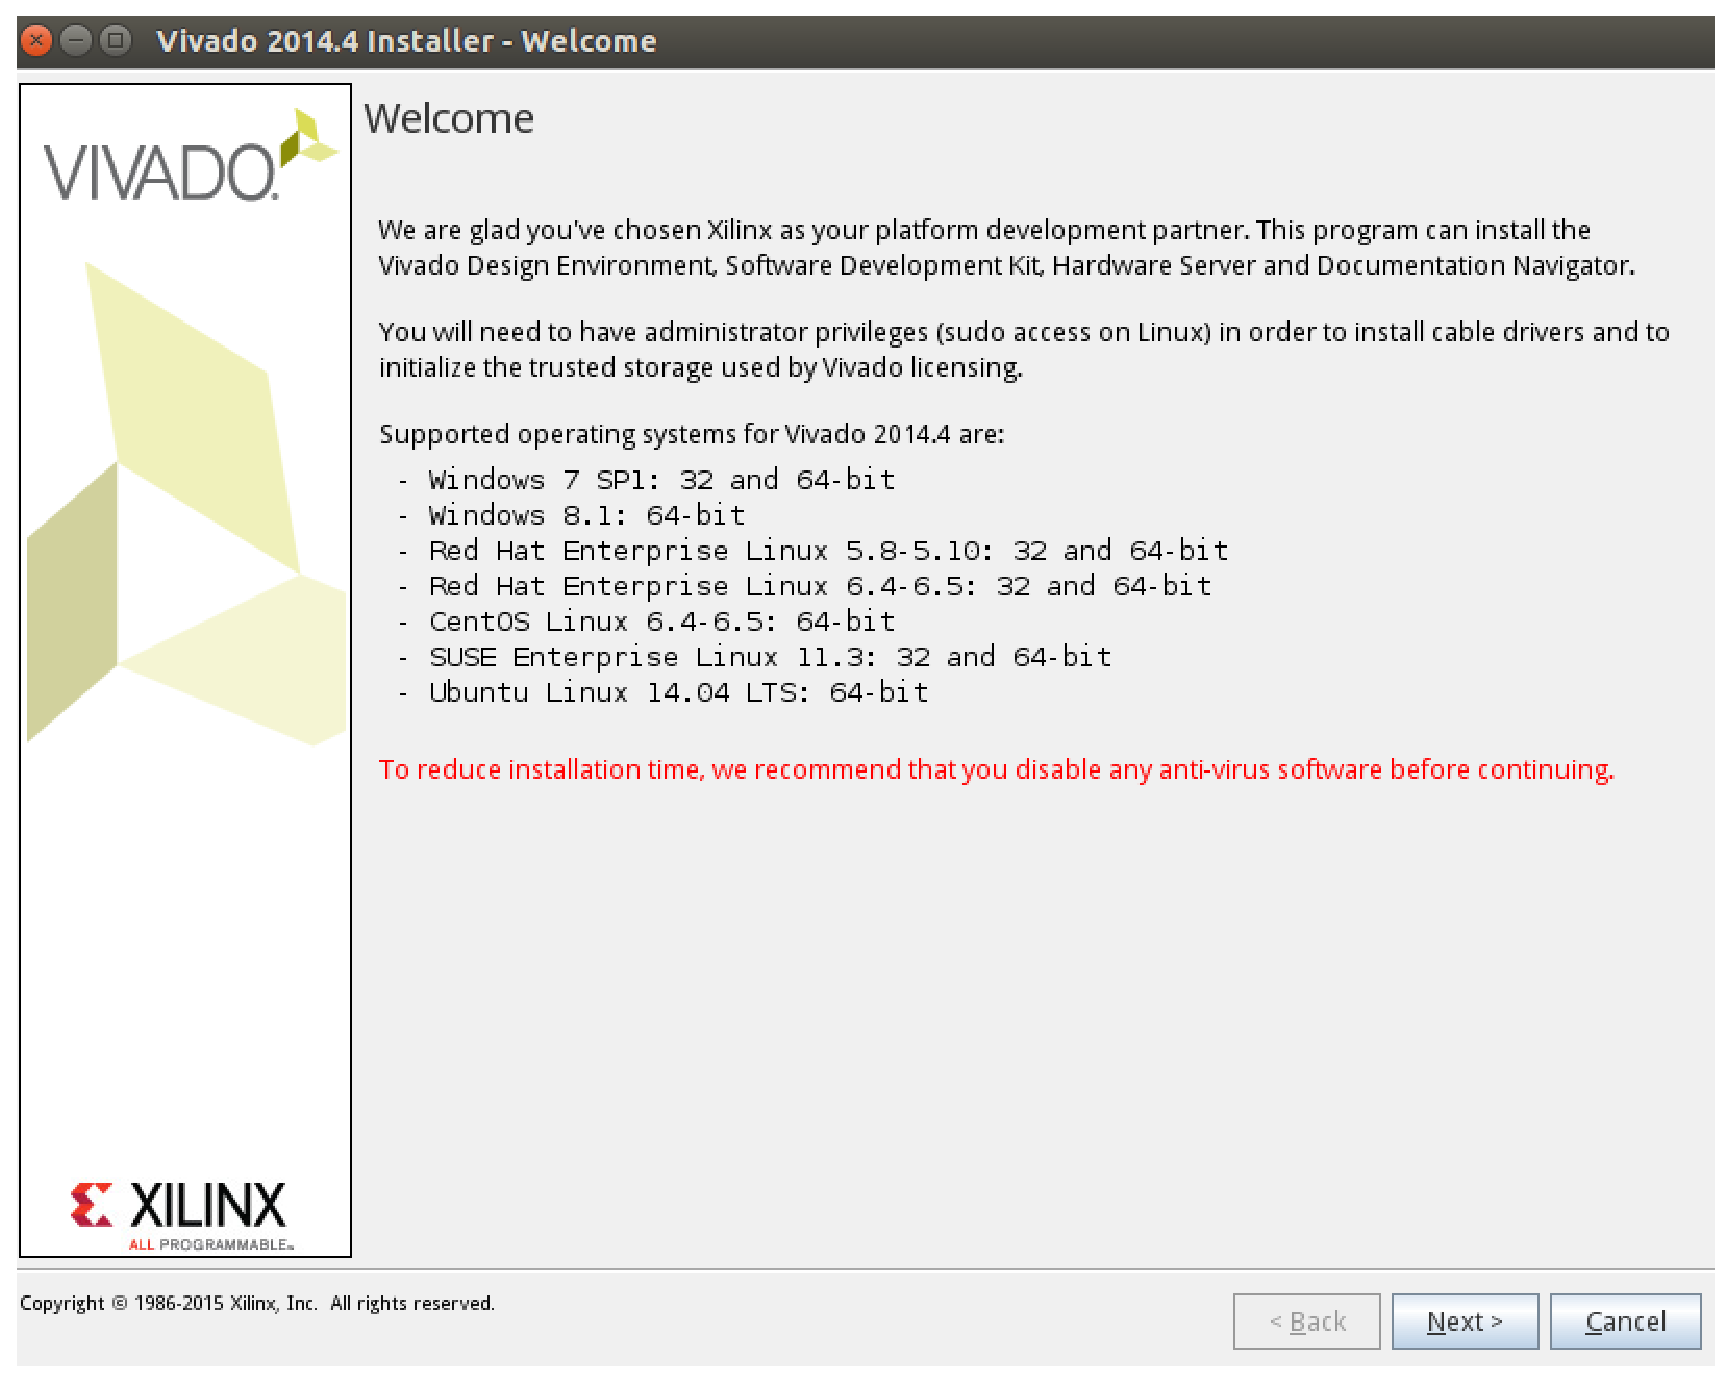
\includegraphics[width=0.8\textwidth, height=0.4\textwidth]{./images/vivado-1.eps}
	\caption{Procedure Vivado installation}
	\label{fig:viva_install_1} 
\end{figure}	

\begin{figure}[h!]
	\centering
	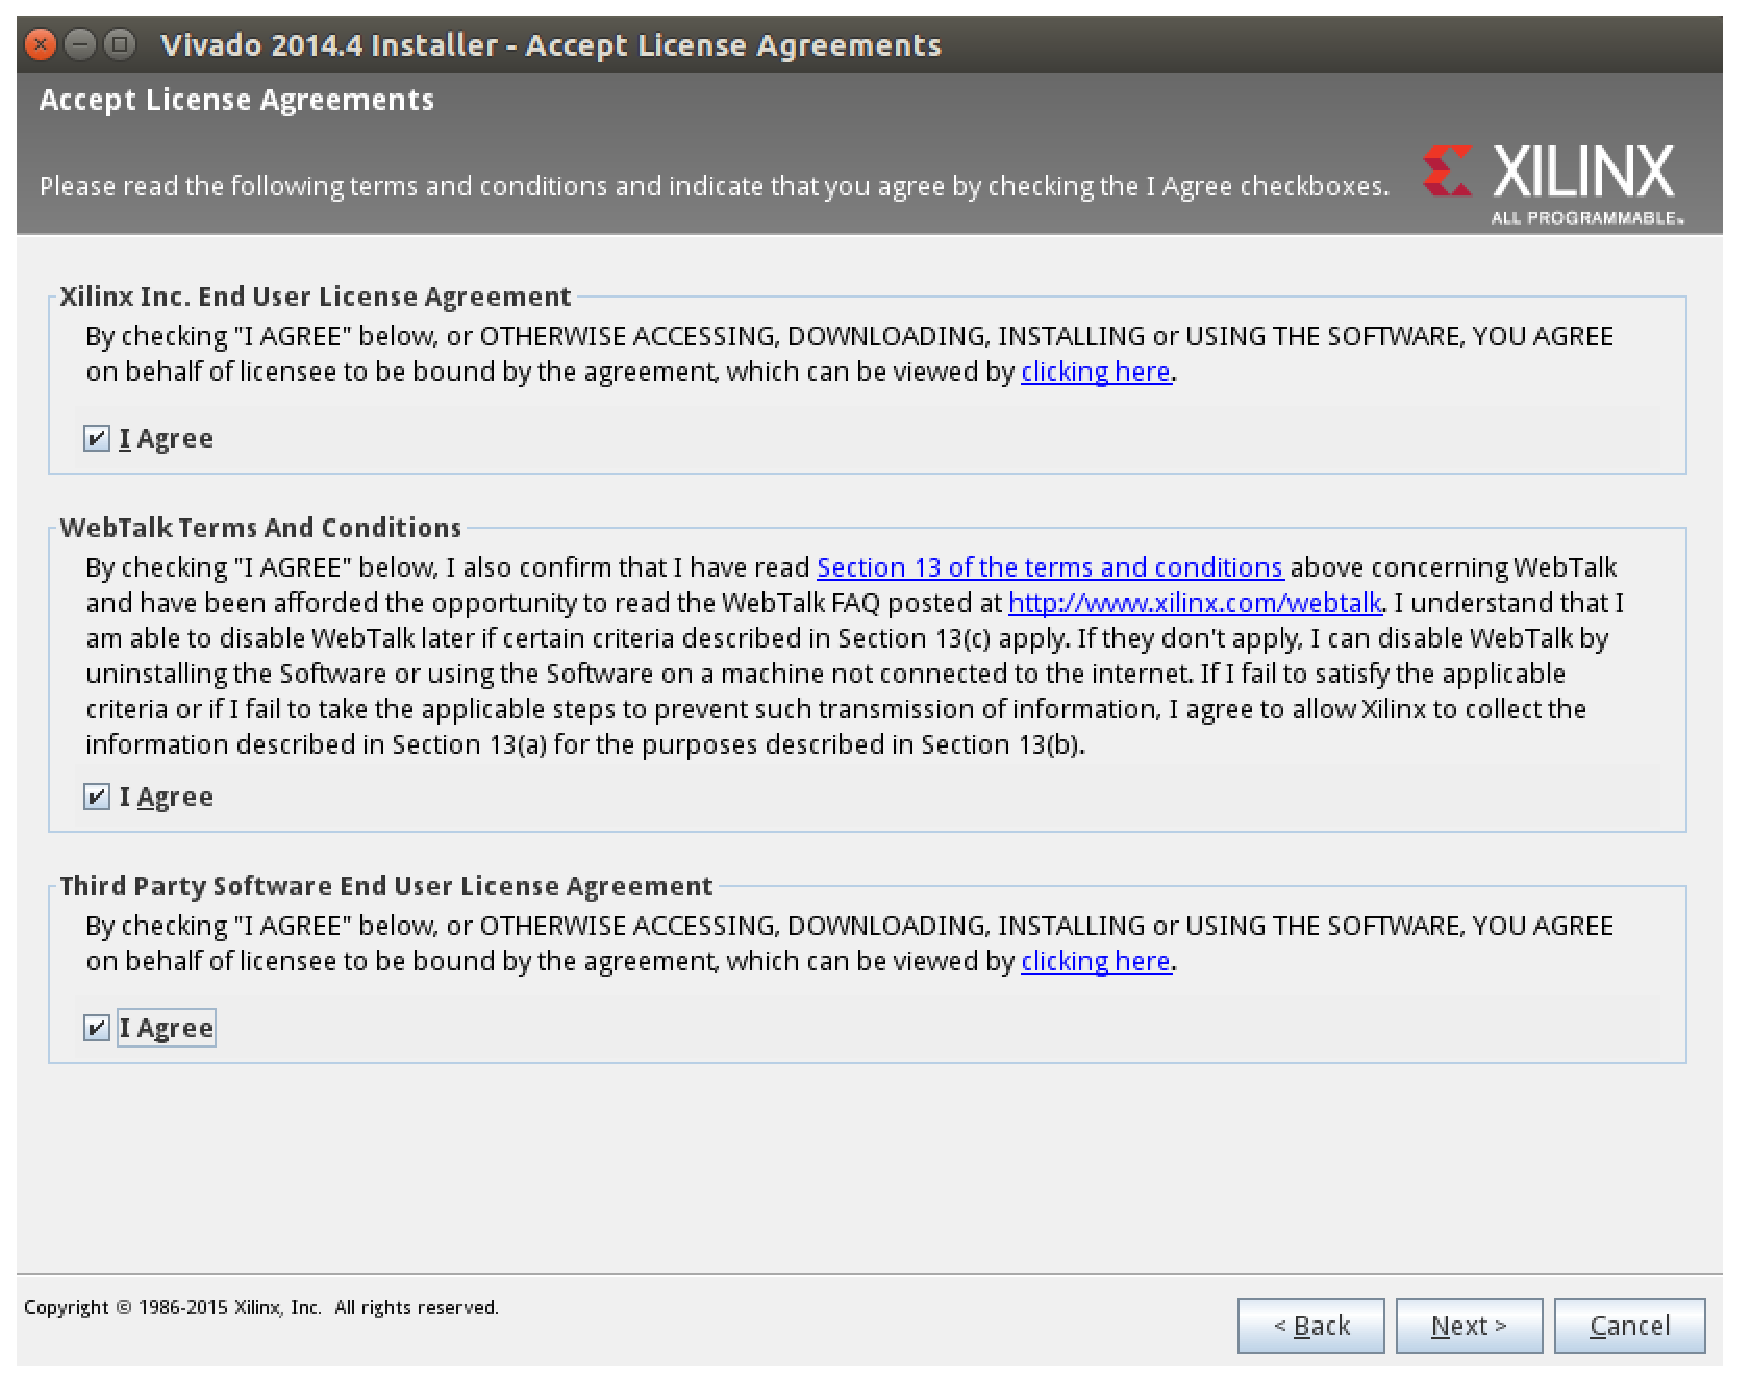
\includegraphics[width=0.8\textwidth, height=0.4\textwidth]{./images/vivado-2.eps}
	\caption{Procedure Vivado installation}
	\label{fig:viva_install_2} 
\end{figure}	


\begin{figure}[h!]
	\centering
	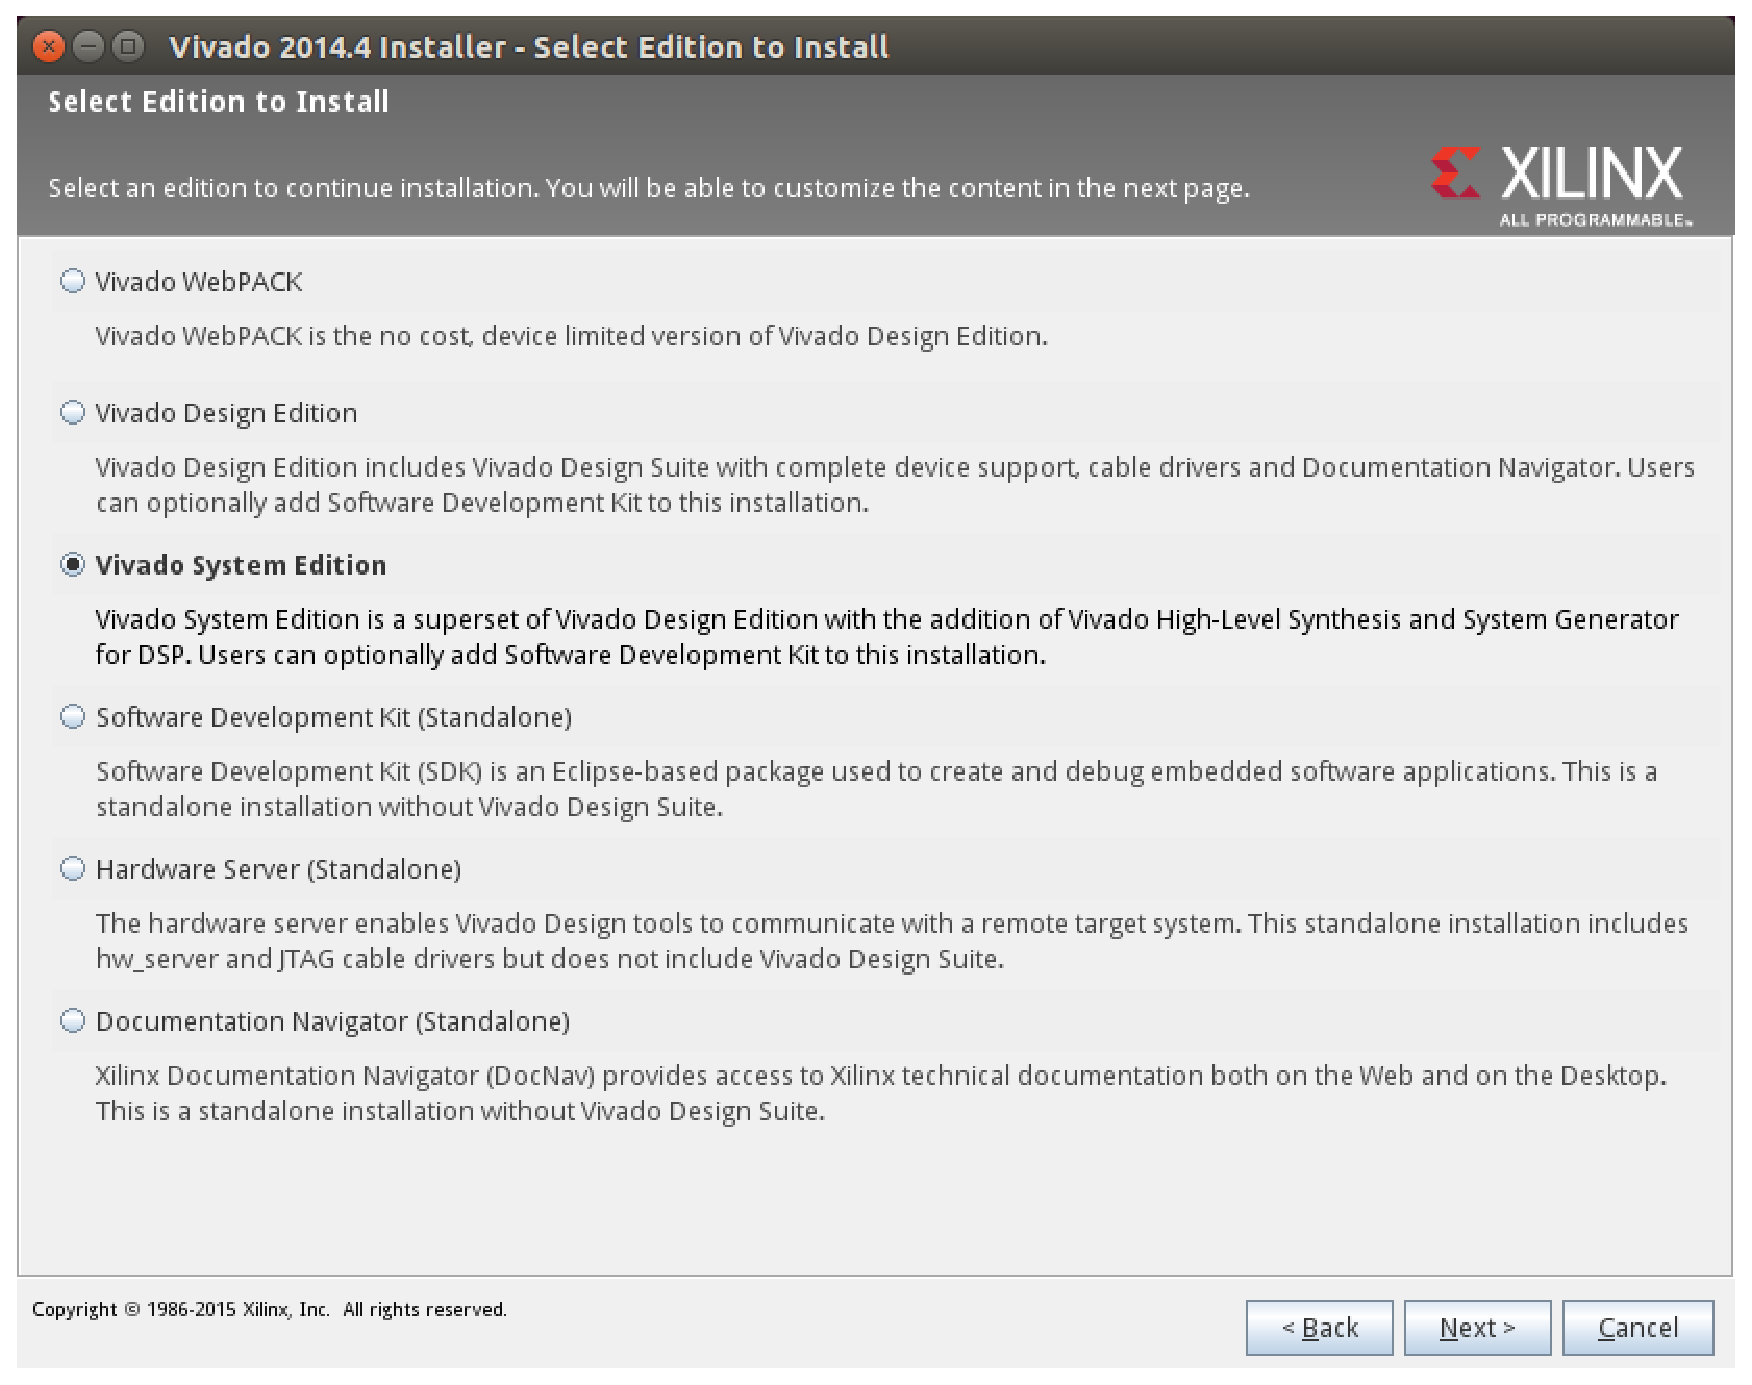
\includegraphics[width=0.8\textwidth, height=0.4\textwidth]{./images/vivado-3.eps}
	\caption{Procedure Vivado installation}
	\label{fig:viva_install_3} 
\end{figure}	

\begin{figure}[h!]
	\centering
	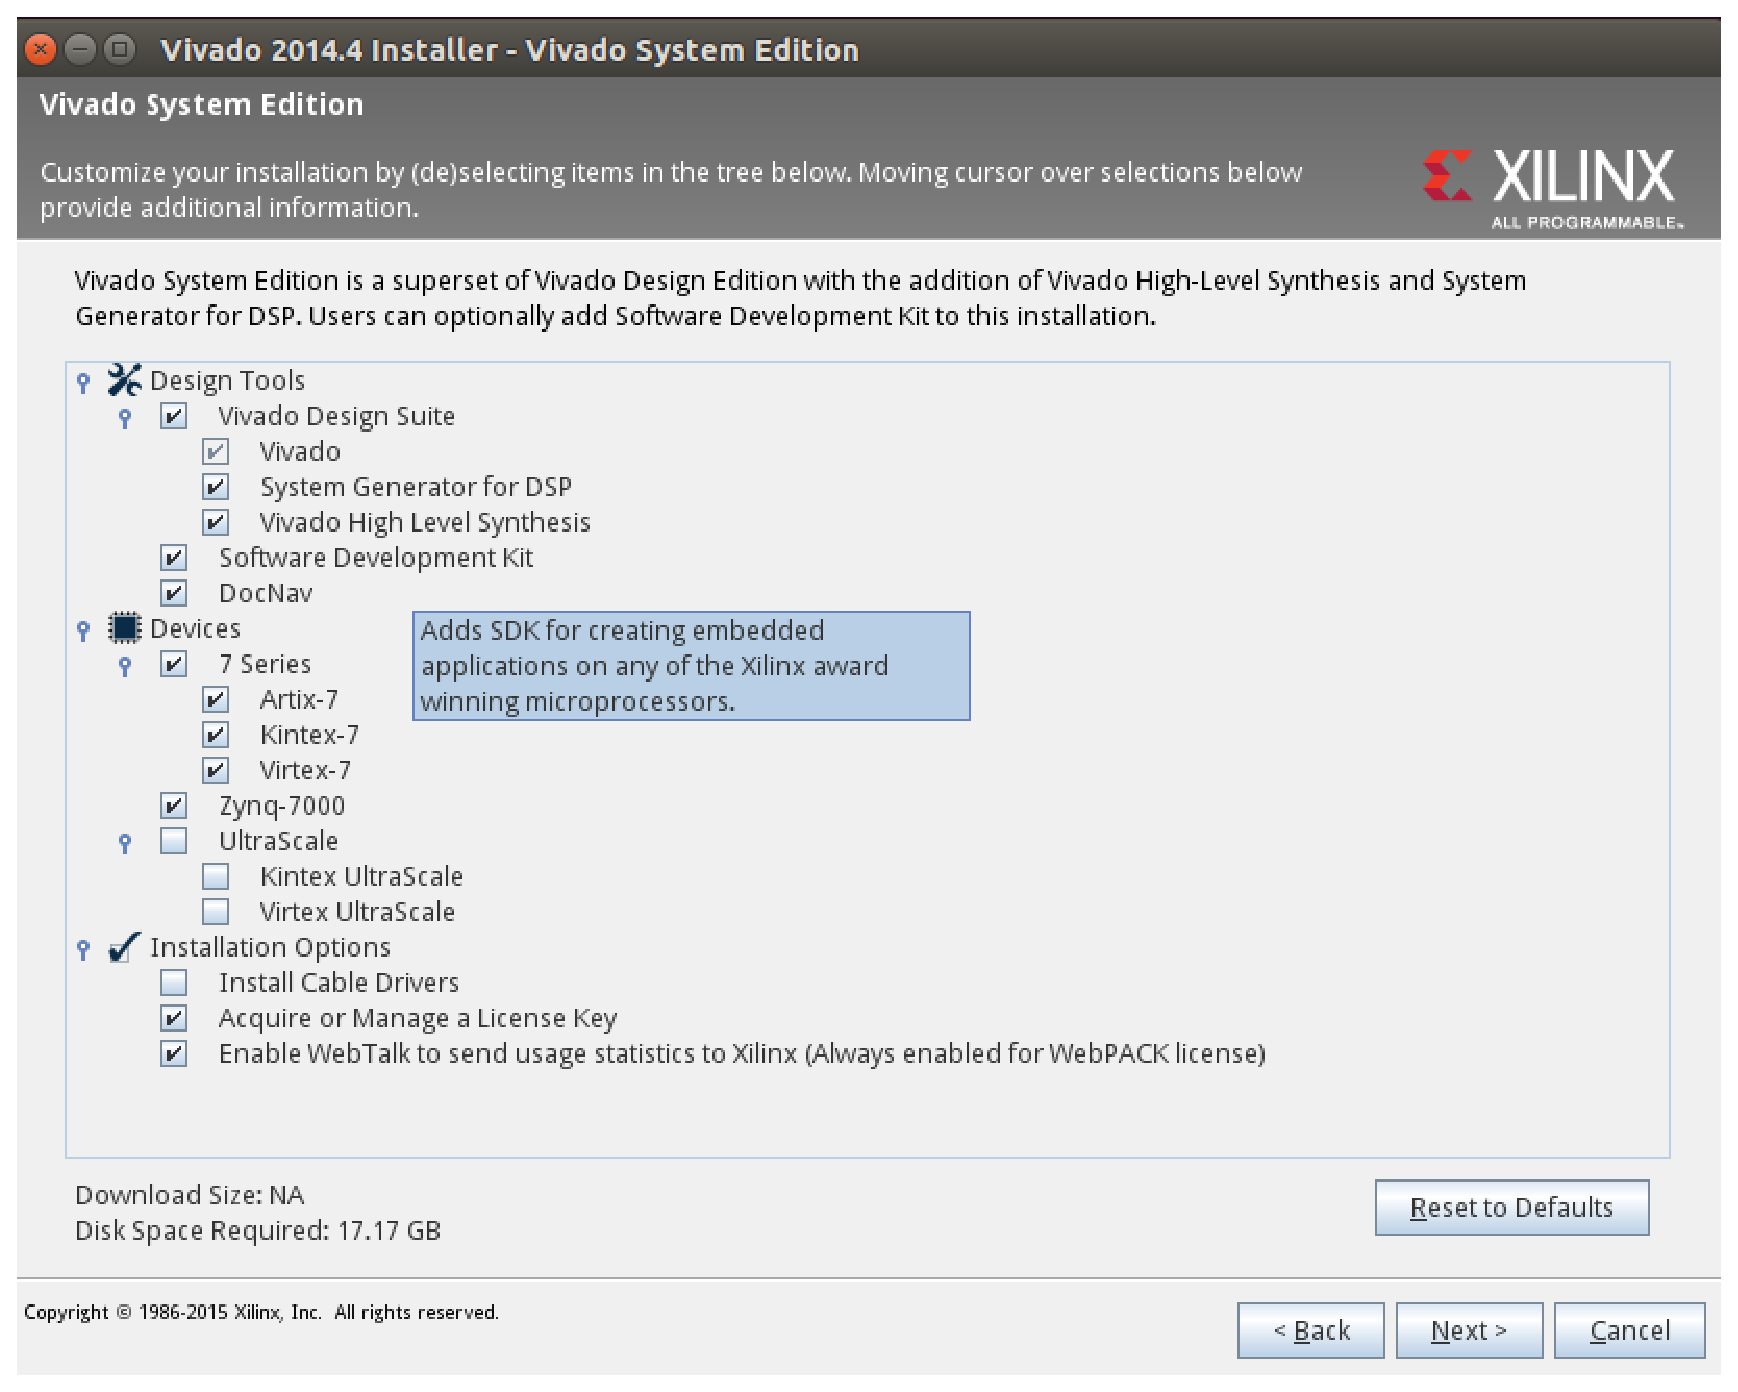
\includegraphics[width=0.8\textwidth, height=0.4\textwidth]{./images/vivado-4.eps}
	\caption{Procedure Vivado installation}
	\label{fig:viva_install_4} 
\end{figure}	

\begin{figure}[h!]
	\centering
	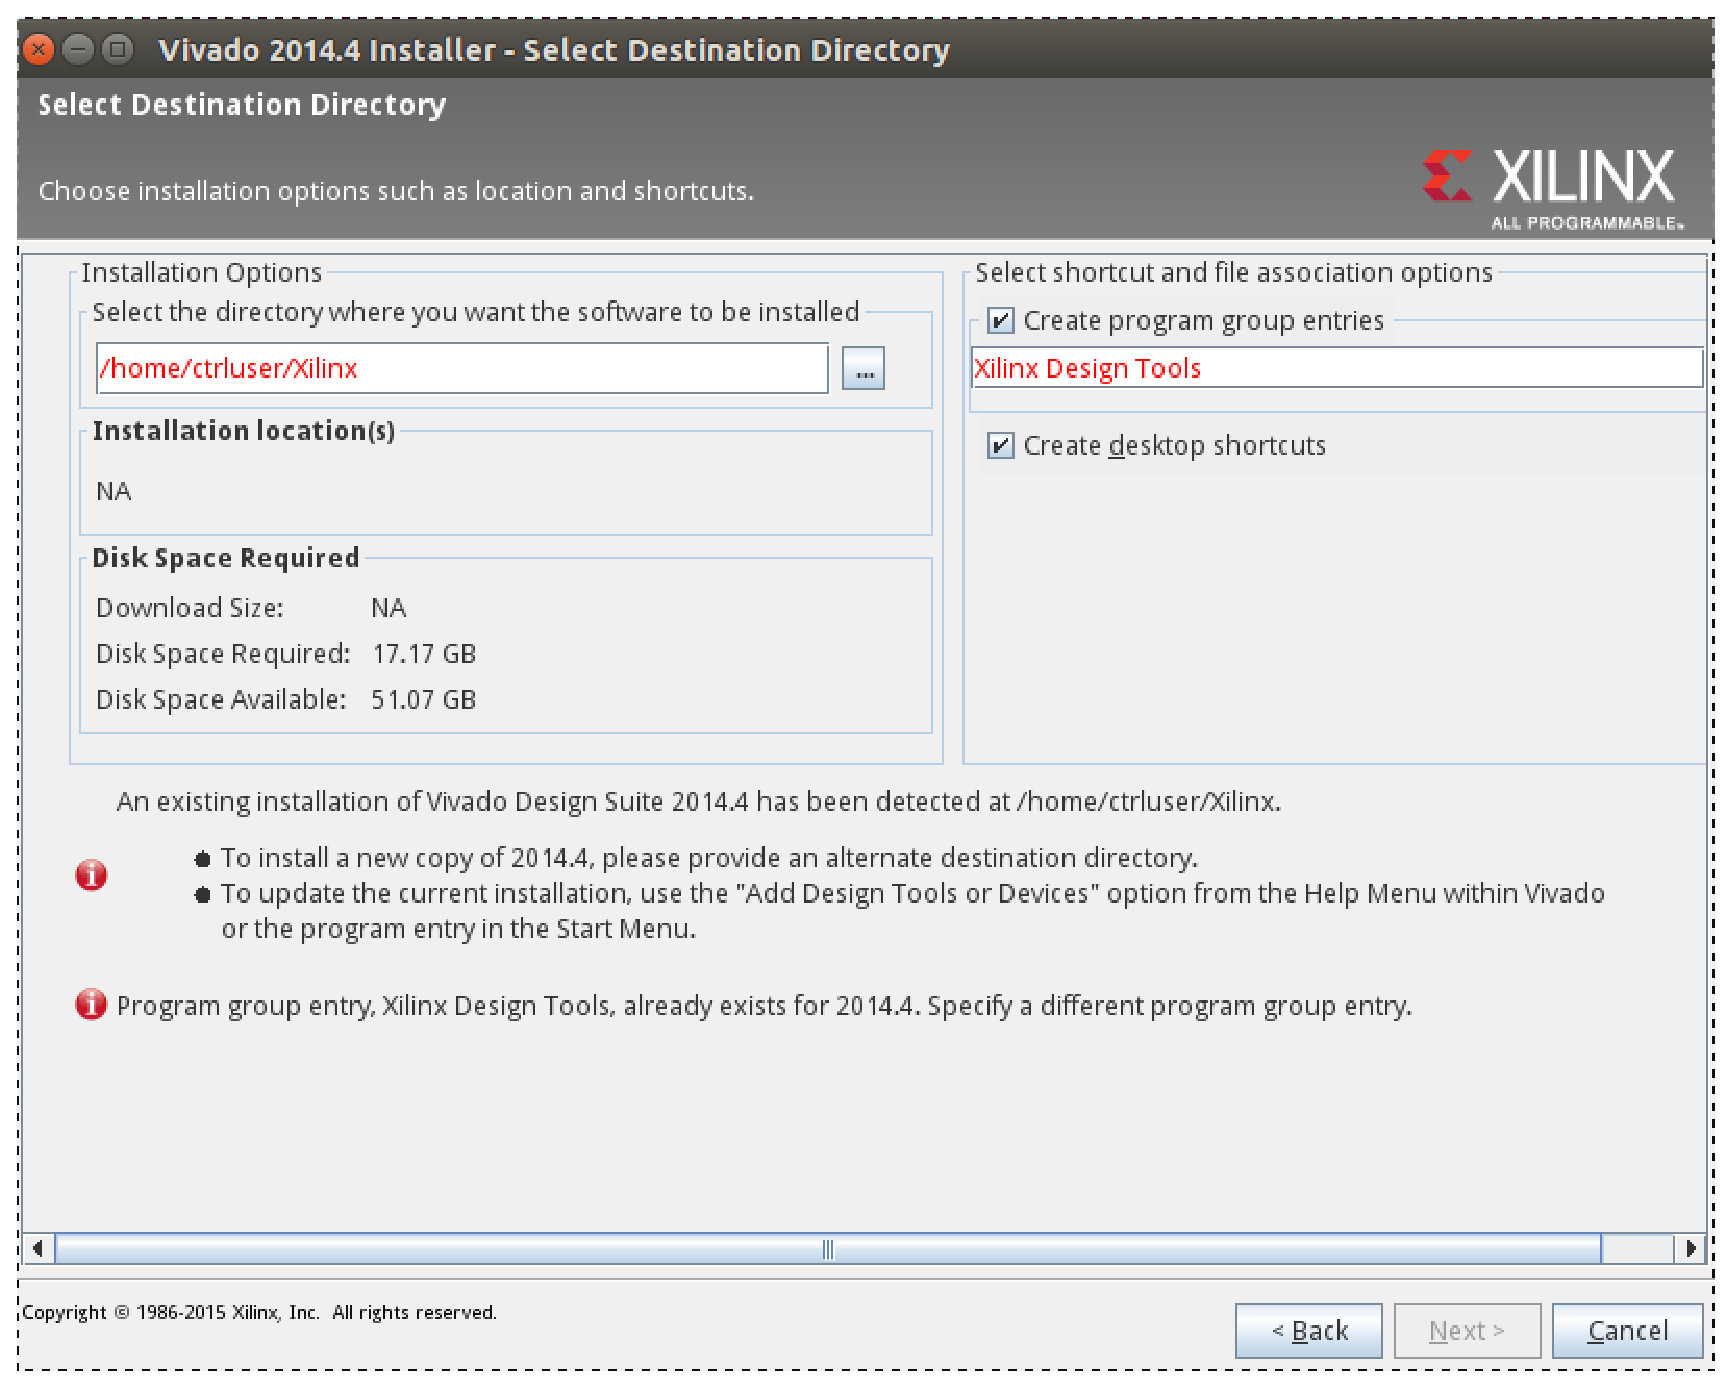
\includegraphics[width=0.8\textwidth, height=0.4\textwidth]{./images/vivado-5.eps}
	\caption{Procedure Vivado installation}
	\label{fig:viva_install_5} 
\end{figure}	

\begin{figure}[h!]
	\centering
	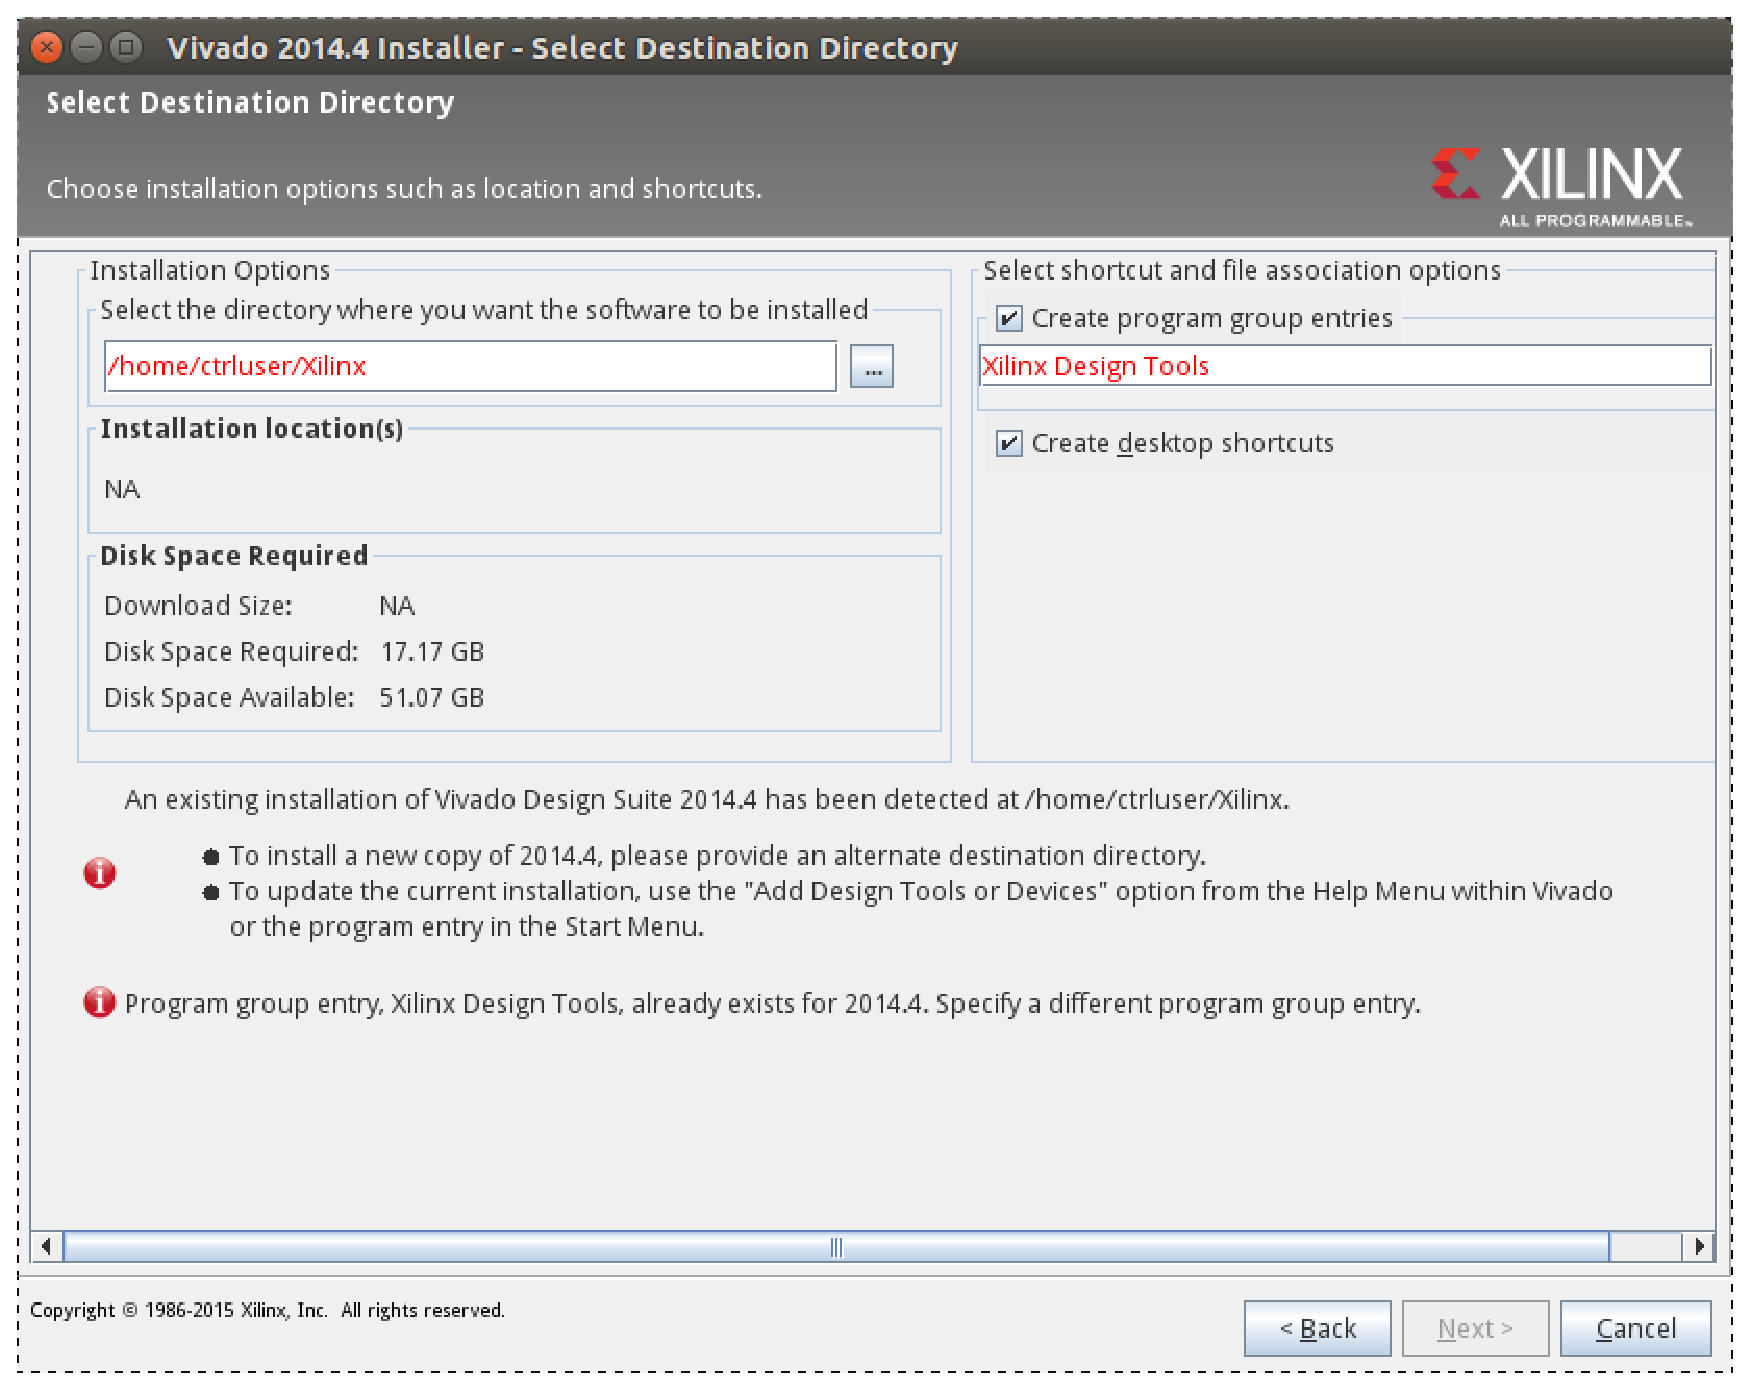
\includegraphics[width=0.8\textwidth, height=0.4\textwidth]{./images/vivado-6.eps}
	\caption{Procedure Vivado installation}
	\label{fig:viva_install_6} 
\end{figure}	

\begin{figure}[h!]
	\centering
	\includegraphics[width=0.8\textwidth, height=0.4\textwidth]{./images/vivado-7.eps}
	\caption{Procedure Vivado installation}
	\label{fig:viva_install_7} 
\end{figure}

\begin{figure}[h!]
	\centering
	
\includegraphics[width=0.8\textwidth, height=0.4\textwidth]{./images/vivado-8.eps}
	\caption{Procedure Vivado installation}
	\label{fig:viva_install_8} 
\end{figure}

\begin{figure}[h!]
	\centering
	\includegraphics[width=0.8\textwidth, height=0.4\textwidth]{./images/vivado-9.eps}
	\caption{Procedure Vivado installation}
	\label{fig:viva_install_9} 
\end{figure}

\clearpage

License Manager를 이용하여 Node Locked 라이센스를 입력하여 설정을 완료한다. Xilinx Site의 회원 ID:silee7103, Password:dev~d 이다.

\chapter{Ubuntu 14.04 LTS 64bit 설정}
RAON에서 사용되는 표준 OS로 Debian을 사용하고 있지만. Xilinx Vivado를 이용항 FPGA를 개발하기 위하여는 Vivado 의 동작을 보장하는 OS 선택이 바람직하다고 생각한다. Ubuntu를 사용하여도 EPICS를 설치 자동화 스크립트를 사용 가능하다.
단, 아래와 같이 git clone으로 받은 자동화 스크립트에서 require\_packages.sh의 OS 버전체크 부분을 수정하거나 아래와 같이 주석을 한다.


\begin{lstlisting}[style=termstyle]
dist=`lsb_release -c | awk '{print $2}'`
#echo $version
## add logic to install some packa
#case "$dist" in
#    wheezy)
##      echo "Wheezy">&2
##      filename_version="package_list_wheezy"
#       ;;
#    jessie)
##      echo "Jessie">&2
##      package_filename="package_list_jessie"
#       ;;
#    *)
#       echo >&2
#       echo "Doesn't support $dist" >&2
#       echo >&2
#       exit 0
#       ;;
#esac
\end{lstlisting}

Ubuntu의 기본 쉘은 dash 쉘을 사용하므로, 아래와 같이 dash 기본 설정을 해제한다.
\begin{lstlisting}[style=termstyle]
sudo dpkg-reconfigure dash
select no
\end{lstlisting}

Ubuntu 64bit에서 추가적인 라이브러리를 아래와 같이 설치한다.
\begin{lstlisting}[style=termstyle]
sudo aptitude install lib32z1 lib32ncurses5 lib32bz2-1.0
\end{lstlisting}


\chapter{System Generator 설정}
System Generator는 Xilinx사에서 Matlab-Simulink를 활용할 수 있는 Xilinx 툴박스를 제공한다. 따라서, 바탕화면에 설정된 System Generator를 더블클릭 하거나 Xilinx 실행 폴더 bin의 sysgen을 실행하면 Xilinx 툴박스 라이브러리 경로가 환경변수로 입력된 후 Matlab이 실행된다. 올바른 설정이 되었다면 아래화면에서 처럼 Simunlink Libraries 창에 "Xilinx Blockset"과 "Xilinx Reference Blockset"이 생성되어 나타난다. 기본 Path 설정이 맞질 않는 다면 아래화면은 실행 되지 않을 것이다.

\begin{figure}[h!]
	\centering
	\includegraphics[width=0.8\textwidth, height=0.4\textwidth]{./images/sysgen-1.eps}
	\caption{System Generator Configuration}
	\label{fig:sysgen_1} 
\end{figure}

올바른 실행이 되질 않는다면 다음 두개의 파일을 수정하여야 한다. \\
Xilinx/Vivado/2014.4/data/sysgen/.matlab7rc.sh 파일에서  MATLAB\_UTIL\_DIR 변수에 Matlab util 디렉토리 경로를 맞추어 설정한다.
\begin{lstlisting}[style=termstyle]
-->~/Xilinx/Vivado/2014.4/data/sysgen/.matlab7rc.sh
echo "Configuring MATLAB runtime using Xilinx Supplied .matlab7rc.sh file copied to your home directory"
MATLAB_UTIL_DIR=/usr/local/MATLAB/R2014a/bin/util
\end{lstlisting}

Xilinx/Vivado/2014.4/bin/sysgen 스크립트 파일에서 XILINX\_MATLAB\_ROOT\_PATH 에 아래와 같이 해당 경로를 맞추어 설정한다.

\begin{lstlisting}[style=termstyle]
451   #Clean up before proceeding to setup environment
452   XILINX_MATLAB_ROOT_PATH=/usr/local/MATLAB/R2014a
\end{lstlisting}

이러한 구성이 완료되었다면 Xilinx 환경변수 settings64.sh를 source 한 후 sysgen을 실행 시켜 그림 \ref{fig:sysgen_1}과 같이 나타남을 확인한다.

이로써 Matlab-Simulink with Vivado-SystemGenerator를 이용하기 위한 환경설정이 완료되었다.

이후 Good luck...


\bibliographystyle{unsrtnat}
\bibliography{./refs}

\end{document}

